% !TeX root = responseletter.tex

\noindent\textbf{--\ Response to Reviewer $\sharp3$}\\

\textsf{This paper first developed an analytical model based on queueing theory for evaluating the QoS of a data center by optimizing three conflicting objectives with regard to energy consumption and QoS. Then, based on the proposed three-objective optimization model, a domain-specific evolutionary optimization framework featuring a tailored solution representation and a constraint-aware initialization operator was proposed for finding the optimal placement of virtual network functions in a data center. Finally, the experimental results validated the efficiency and accuracy of the proposed QoS model as well as the effectiveness of the tailored algorithms for virtual network function placement problems at various scales.}

\textsf{Generally speaking, the topic of this work is interesting with good writing.}

\textcolor{blue}{\textbf{\textit{Reply}: We appreciate the reviewer’s positive affirmation of the contributions of our work.}}\\

\noindent\textsf{However, this paper could not be published if the following comments cannot be solved very carefully in the future version.}

\begin{enumerate}
      \item\textsf{The appendix files are missed in the current version.}\\
            \textcolor{blue}{\textbf{\textit{Reply}: We apologize for this mistake. The link to the appendix has now been corrected.}} \\

      \item\textsf{In the introduction part, the authors stated that “Both operations can be seamlessly incorporated into any evolutionary multi-objective optimization (EMO) algorithm”, however, in the experimental results, they did not validate this and they only incorporated these strategies into NSGA-II. What’s the effect by incorporating these strategies into MOEA/D? or other MOEAs. The authors should validate this in their experiments.}\\
            \textcolor{blue}{\textbf{\textit{Reply}: We thank the reviewer for this suggestion. We have added a dedicated subsection that illustrates the results of implementing the operators in three seminal MOEAs: NSGA-II, MOEA/D and IBEA.}}\\
            \textcolor{blue}{
                  To illustrate that our operators can be integrated into any MOEA framework, we compare the quality of solutions obtained when different MOEAs are used with our proposed operators. Specifically, we integrated our proposed operators into three state of the art MOEAs: NSGA-II \cite{DebAPM02}, MOEA/D \cite{ZhangL07} and IBEA \cite{ZitzlerK04}. \\In our experiments, we generate $30$ VNFPP instances for six data centers with different sizes. To compare the performance of different algorithms, we use the QoS model developed in~\pref{sec:system_model} to evaluate the objective functions of the solutions obtained by different algorithms and use the HV indicator as the performance measure.
            }
            \begin{figure}[h!]
                  \centering
                  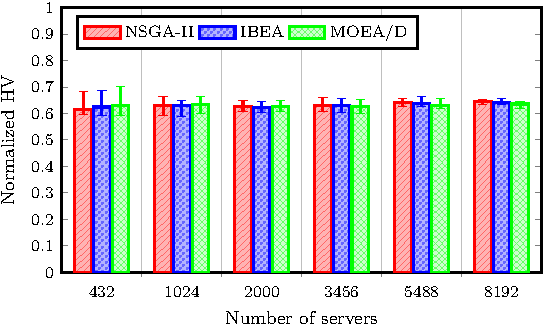
\includegraphics[width=.7\columnwidth]{figs/moeas-crop}
                  \caption{The lower quartile, median, and upper quartile of the hyper-volume of the population for different MOEAs on 30 VNFPP instances.}
                  \label{fig:moea_comparison}
            \end{figure}\\
            \textcolor{blue}{
                  The results of this test are illustrated in~\pref{fig:moea_comparison}. We found that all algorithm performed similarly, with no algorithm performing consistently significantly better than any other. Given all algorithms performed similarly, we have selected NSGA-II for use in future tests based on its widespread adoption in the literature.
                  \textbf{(Page x, highlighted in \textcolor{red}{red} color.)} }

      \item\textsf{My biggest concern is the difference between the proposed method with the author’s previous works. Although the authors tried to illustrate the difference between the proposed algorithm with their previous work [16]. E.g. compared with the proposed work, the work of [16] did not consider the packet loss and is only applicable to small-scale VNFPPs. Could you explain these in detail? E.g. What’s the technique difference between these two works? E.g. Why [16] can only applicable to small-scale VNFPPs? Why the current method can solve the large-scale VNFPPs? }\\
            \textcolor{blue}{\textbf{\textit{Reply}: We thank the reviewer for this comment. There are several key differences between the two algorithms. In our revised manuscript we have elaborated on these distinctions.}}\\
            \textcolor{blue}{\textit{``To the best of our knowledge, our previous work~\cite{TODO} is the only one that combines meta-heuristics with a queueing model for VNFPP. We used a simple solution representation where each solution is represented as a string of VNFs and proposed custom mutation and initialization operators to improve the chances of placing at least one instance of each VNF. It also used a simple queuing model that calculates the latency and energy consumption but does not consider packet loss. In our current work, we propose a more advanced solution representation that allows for more diverse solutions without requiring custom genetic operators. Further, we show that this new representation is simple to extend to complex constraints. Finally, we improve upon the model to consider packet loss and show how this significantly affects the quality of solutions."} \textbf{(Page x, highlighted in \textcolor{red}{red} color.)}}\\

            \textsf{In addition, the authors should compare them in experimental part with the aim to show the advantages of the proposed methods.}\\
            \textcolor{blue}{\textbf{\textit{Reply}: We thank the reviewer for this suggestion. In our revised manuscript we have included our previously proposed algorithm in our comparison.}}\\
            \textcolor{blue}{\textit{``$\cdots$TODO"} \textbf{(Page x, highlighted in \textcolor{red}{red} color.)}}\\

            \textsf{At last, I found that the authors has published a recent work in EMO 2021 named “Parallel Algorithms for the Multiobjective Virtual Network Function Placement Problem”. What’s the main differences between this work and the proposed method? }\\
            \textcolor{blue}{\textbf{\textit{Reply}: We thank the reviewer for this comment. The aforementioned work submitted to EMO and a related work 'Routing-Led Placement of VNFs in Arbitrary Networks' published in WCCI both build upon and reference the paper we are submitting to this journal. Specifically, the WCCI paper explores how this journal paper can be extended to arbitrary networks and the EMO paper applies parallel MOEAs to solve VNFPPs in arbitrary graphs. This journal paper is the keystone work of both of these papers. In particular, both conference papers reference the model, initialization, solution representation and results of this journal paper. Further, although the conference papers above are reliant on this journal paper, they do not restate the concepts introduced in this paper.}}\\

      \item\textsf{In related work part, the sentence “They first pre-processed the network topology to find the most influential nodes according to the Katz centrality.” where the Katz centrality should be followed with a reference.}\\
            \textcolor{blue}{\textbf{\textit{Reply}: We thank the reviewer for identifying this issue and have added a reference to the seminal work \textit{'A new status index derived from sociometric analysis'} by Leo Katz, where the Katz centrality was first proposed.}}\\
            \textcolor{blue}{\textit{``...They first pre-processed the network topology to find the most influential nodes according to the Katz centrality \cite{TODO}."} \textbf{(Page x, highlighted in \textcolor{red}{red} color.)}}\\

      \item\textsf{When the authors presented the proposed Genotype-Phenotype Solution Representation, the authors had better give a illustrated example to show what the solution looks like. Currently, it is somehow abstract.}\\
            \textcolor{blue}{\textbf{\textit{Reply}: We thank the reviewer for this comment. In the updated manuscript we have included a figure illustrating the genotype-phenotype solution representation.}}\\
            \textcolor{blue}{\textbf{(Page x, highlighted in \textcolor{red}{red} color.)}}

      \item\textsf{There are some unclear places when introducing the experimental results. For example, why the Simulation benchmark in Fig. 5 are zero in terms of Latency, Packet Loss and Energy?}\\
            \textcolor{blue}{\textbf{\textit{Reply}: We thank the reviewer for this comment. To clarify, these metrics are only zero when the average arrival rate is zero. This would occur if the data center was not in use.}}\\

            \textsf{What’s the meaning of nodes with different colors in Fig. 6?}\\
            \textcolor{blue}{\textbf{\textit{Reply}: We thank the reviewer for this comment. In these figures, each node represents a solution from the final population. The colours on the figure relate to the latency of each solution but are intended to help the reader to distinguish between solutions. We have improved the caption of each of the relevant figures to better reflect these details, e.g. the caption of Fig. 7 now reads:}}\\
            \textcolor{blue}{\textit{``An illustrative example of the objective values of the solutions found by NSGA-II using our proposed model and
            models from the literature. More diverse solutions with lower objective values indicate more appropriate models."} \textbf{(Page x, highlighted in \textcolor{red}{red} color.)}}

\end{enumerate}

\clearpage
